\documentclass{article}%
\usepackage[T1]{fontenc}%
\usepackage[utf8]{inputenc}%
\usepackage{lmodern}%
\usepackage{textcomp}%
\usepackage{lastpage}%
\usepackage[head=40pt,margin=0.5in,bottom=0.6in]{geometry}%
\usepackage{graphicx}%
%
\title{\textbf{Registraron 47 muertes por desnutrición infantil en Monagas}}%
\author{EL NACIONAL WEB}%
\date{20/11/2018}%
%
\begin{document}%
\normalsize%
\maketitle%
\textbf{URL: }%
http://www.el{-}nacional.com/noticias/sociedad/registraron{-}muertes{-}por{-}desnutricion{-}infantil{-}monagas\_260479\newline%
%
\textbf{Periodico: }%
EN, %
ID: %
260479, %
Seccion: %
Sociedad\newline%
%
\textbf{Palabras Claves: }%
Monagas, Sociedad\newline%
%
\textbf{Derecho: }%
2.1%
, Otros Derechos: %
NO\_TIENE%
, Sub Derechos: %
2.1.1%
\newline%
%
\textbf{EP: }%
NO\newline%
\newline%
%
\textbf{\textit{El pasado viernes falleció un menor de un año de edad en el Hospital Universitario Dr. Manuel Núñez Tovar}}%
\newline%
\newline%
%
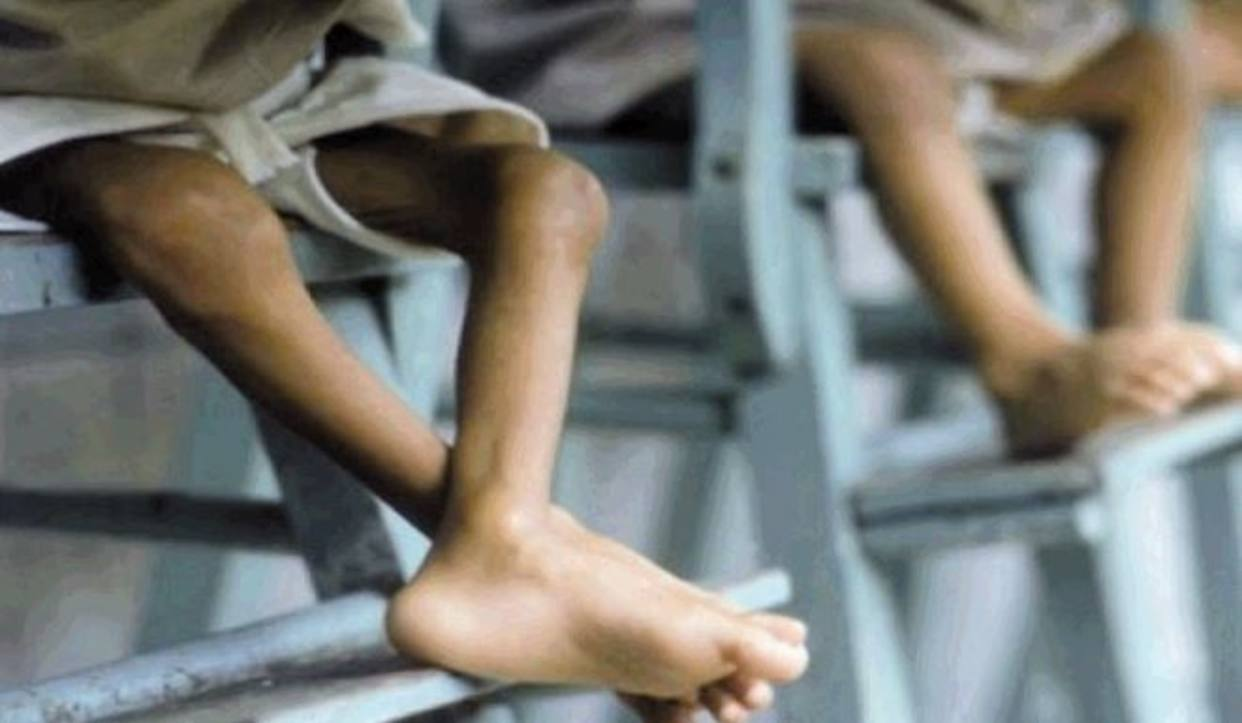
\includegraphics[width=300px]{192.jpg}%
\newline%
%
Yacirka Vásquez, jefa del servicio de emergencia pediátrica del Hospital Universitario Dr. Manuel Núñez Tovar, afirmó que los casos de desnutrición en el estado Monagas provienen de zonas urbanas y que ya no son propios de sitios rurales.%
\newline%
%
El centro de salud registró 47 muertes de infantes por desnutrición durante 2018, de los cuales 70\% de los fallecimientos corresponden a Maturín, capital de la entidad, y ocurrieron entre febrero y julio, reseñó~El Pitazo.%
\newline%
%
El pasado viernes murió un bebé de un año de edad en el centro de salud, el menor estuvo hospitalizado porque se encontraba descompensado y con valores sanguíneos bajos. En la emergencia pediátrica del hospital lo estabilizaron y le dieron de alta.%
\newline%
%
En el centro de salud indicaron que el menor no era alimentado correctamente en su hogar, puesto que solo consumía maicena, agua de arroz o avena, que no aportan los nutrientes necesarios que necesita un lactante.%
\newline%
%
Con información de~El Pitazo%
\newline%
%
\end{document}